\documentclass[aspectratio=169]{beamer}

\usetheme{Madrid}
\usecolortheme{default}
\setbeamertemplate{navigation symbols}{}
\setbeamertemplate{footline}[frame number]
\usepackage{booktabs}
\usepackage{graphicx}
\usepackage{amsmath}

\title{Adaptive Environment Selection for RL-Based LLM Post-Training}
\author{DSAA3053 Course Project}
\date{April 28, 2026}

\begin{document}

\begin{frame}
  \titlepage
\end{frame}

\begin{frame}{Project Track and Research Question}
  \begin{itemize}
    \item Track: Option 1, algorithm development.
    \item Problem: RL post-training mixes Math and Zebra reasoning environments.
    \item Question: can online advantage signals guide environment selection and correct imperfect static difficulty buckets?
    \item Conservative claim: AES shows interpretable adaptive behavior and step-200 gains, while re-bucketing reveals composition drift.
  \end{itemize}
\end{frame}

\begin{frame}{Method: AES Feedback Loop}
  \centering
  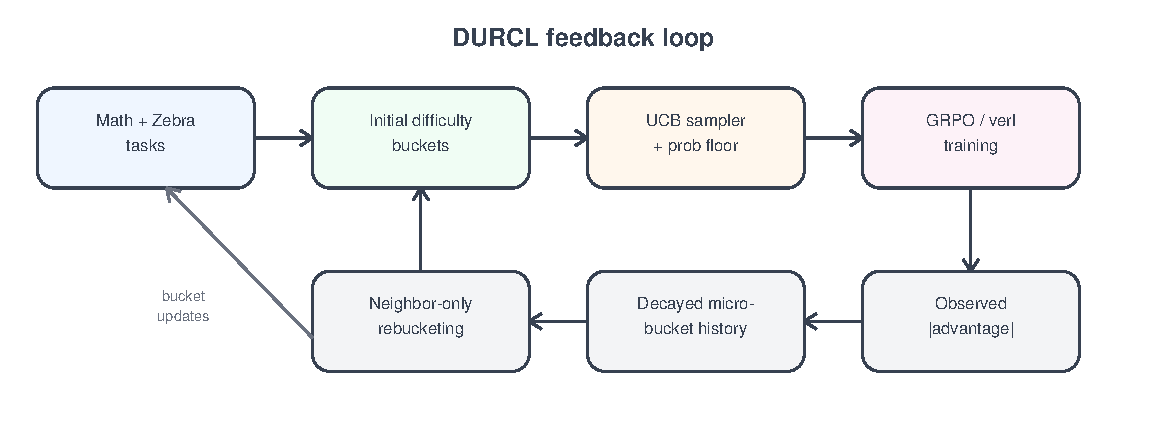
\includegraphics[width=0.95\linewidth]{figures/fig_method_pipeline.pdf}
\end{frame}

\begin{frame}{Scheduler Core}
  \begin{itemize}
    \item Compared with DUMP: replace distribution-level sliding windows with exponential-decay advantage state.
    \item Mixed-data extension: add micro-bucket re-bucketing for Math/Zebra groups with different learning-drift rates.
    \item Initial clusters from difficulty labels or accuracy calibration.
    \item Decayed advantage state:
    \[
      s_i \leftarrow \lambda s_i + (1-\lambda)|A_i|.
    \]
    \item Cluster sampling by UCB plus softmax and probability floor:
    \[
      \mathrm{UCB}_c = v_c + \beta \sqrt{\frac{2\log(N+1)}{n_c+1}}.
    \]
    \item Re-bucketing is local: compare each micro-bucket only with its current and adjacent clusters.
  \end{itemize}
\end{frame}

\begin{frame}{Micro-bucket Rebucketing}
  \begin{itemize}
    \item Split each task--cluster group into micro-buckets; individual samples do not move alone.
    \item Track each micro-bucket by dynamics signature
    \[
      z_g=(\ell_g,s_g),
    \]
    where $\ell_g$ is recent mean $|\hat A|$ and $s_g$ is the fitted slope.
    \item Compare standardized signatures to current-or-adjacent cluster centers:
    \[
      j^\star(g)=\arg\min_{j\in\{k-1,k,k+1\}}\|\tilde z_g-\tilde z_j\|_2^2.
    \]
    \item Apply adjacent mutual swaps only after consistent checks, keeping cluster sizes stable.
  \end{itemize}
\end{frame}

\begin{frame}{Step-200 Result: Math+Zebra}
  \centering
  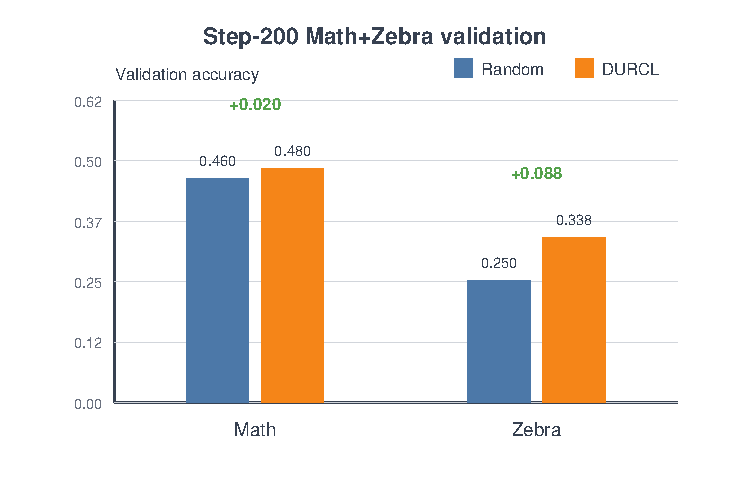
\includegraphics[width=0.62\linewidth]{figures/fig_step200_math_zebra.pdf}
  \vspace{0.5em}

  Scheduler without re-bucketing improves Math by $+0.020$ and Zebra by $+0.088$ over random sampling.
\end{frame}

\begin{frame}{UCB Score Drift}
  \centering
  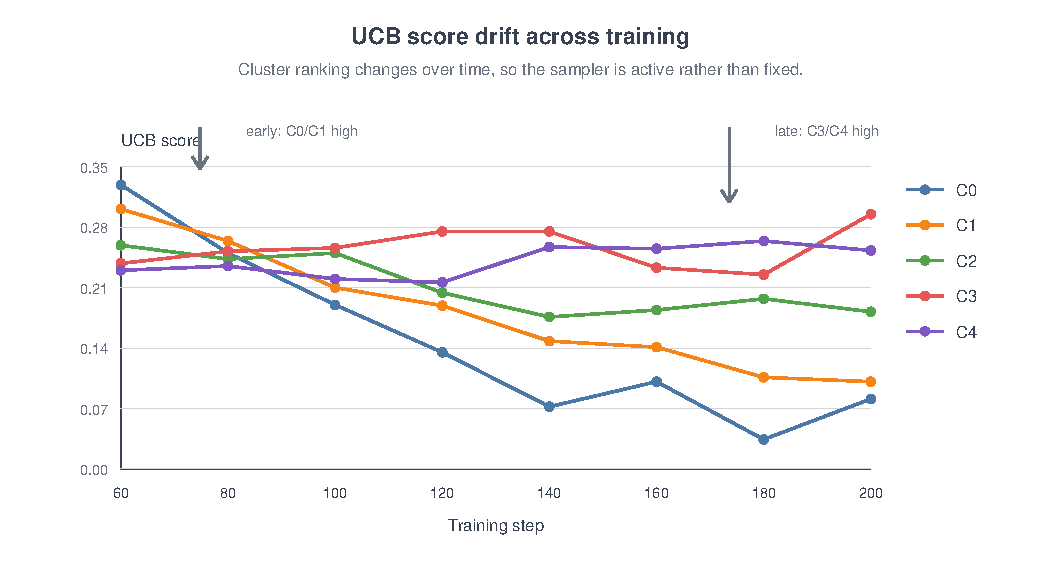
\includegraphics[width=0.72\linewidth]{figures/fig_ucb_score_drift.pdf}

  UCB is active: sampling pressure shifts from C0/C1 early to C3/C4 later. This is useful adaptation, but also a drift signal that must be monitored.
\end{frame}

\begin{frame}{Experiment 1: Initial Accuracy Test}
  \centering
  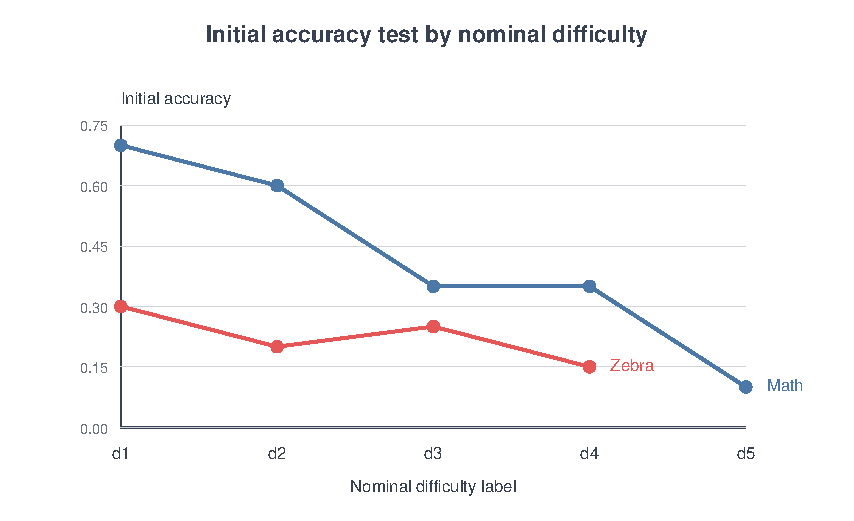
\includegraphics[width=0.60\linewidth]{figures/fig_initial_accuracy_profile.pdf}

  Label-only initialization is coarse: Zebra is non-monotone across difficulty labels, and Math/Zebra have different initial accuracy scales.
\end{frame}

\begin{frame}{Experiment 1: Difficulty Labels Create Composition Drift}
  \centering
  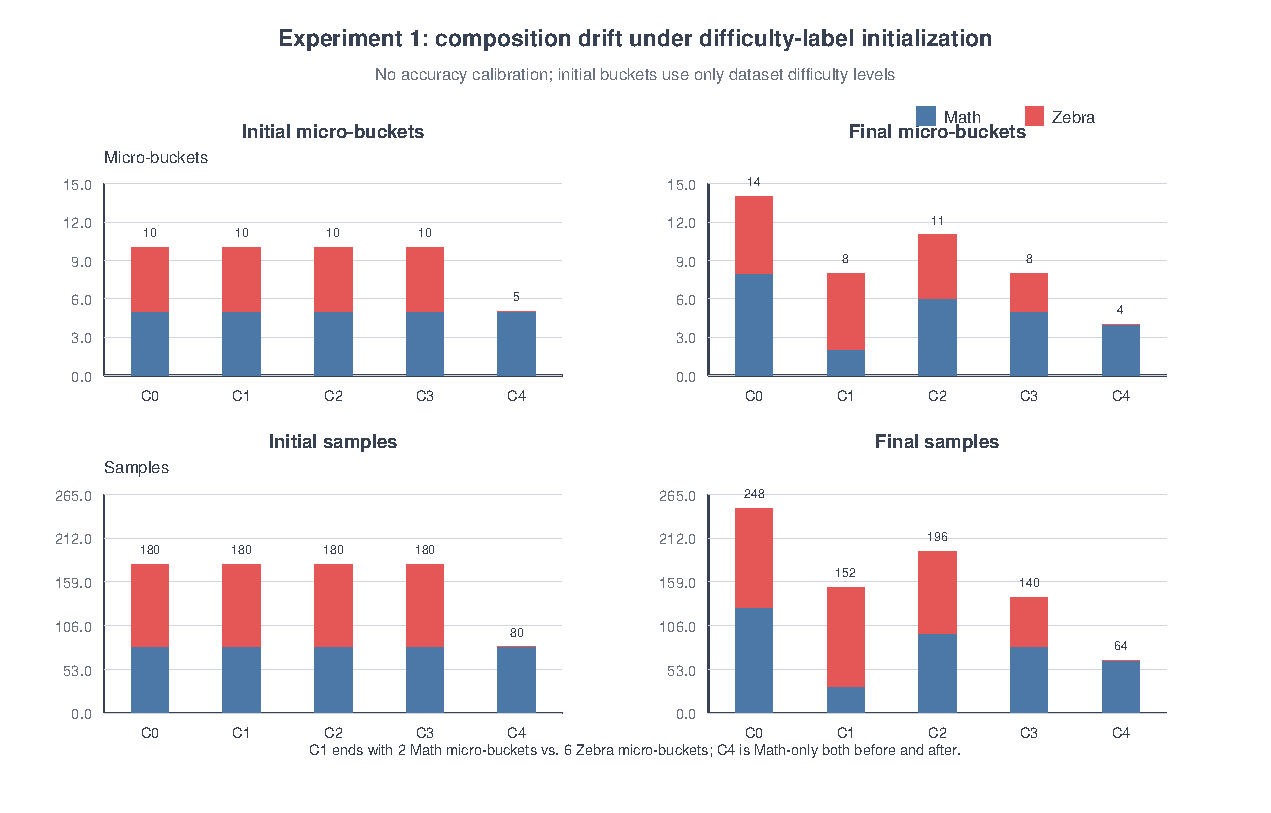
\includegraphics[width=0.62\linewidth]{figures/fig_rebucket_composition.pdf}

  No accuracy calibration: C1 becomes Zebra-heavy, and C4 is Math-only before and after re-bucketing.
\end{frame}

\begin{frame}{Experiment 1: Migration Direction}
  \centering
  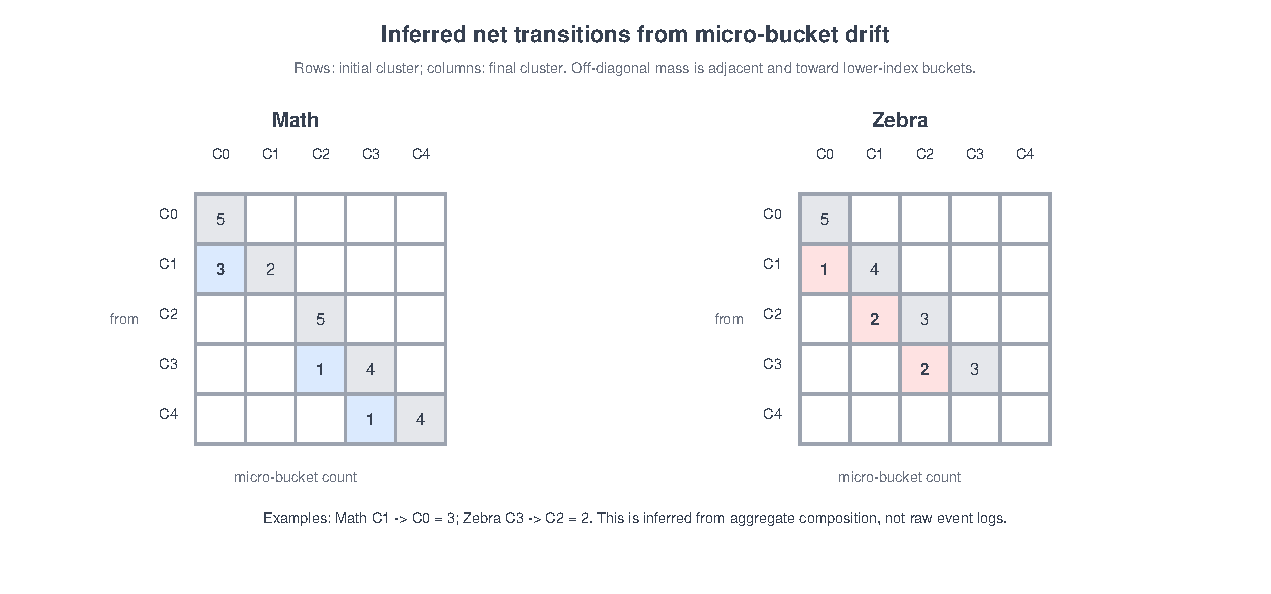
\includegraphics[width=0.78\linewidth]{figures/fig_inferred_transition_matrix.pdf}

  Net movement can be explained by adjacent left moves, e.g. Math C1 $\rightarrow$ C0 and Zebra C3 $\rightarrow$ C2.
\end{frame}

\begin{frame}{Experiment 2: Pending Final Result}
  \begin{itemize}
    \item Setting: accuracy-based initialization.
    \item Comparison: no-rebucket vs. rebucket.
    \item Step: 200.
    \item Status: result not available yet; table is intentionally left pending in the report.
  \end{itemize}
\end{frame}

\begin{frame}{Mechanism Check}
  \centering
  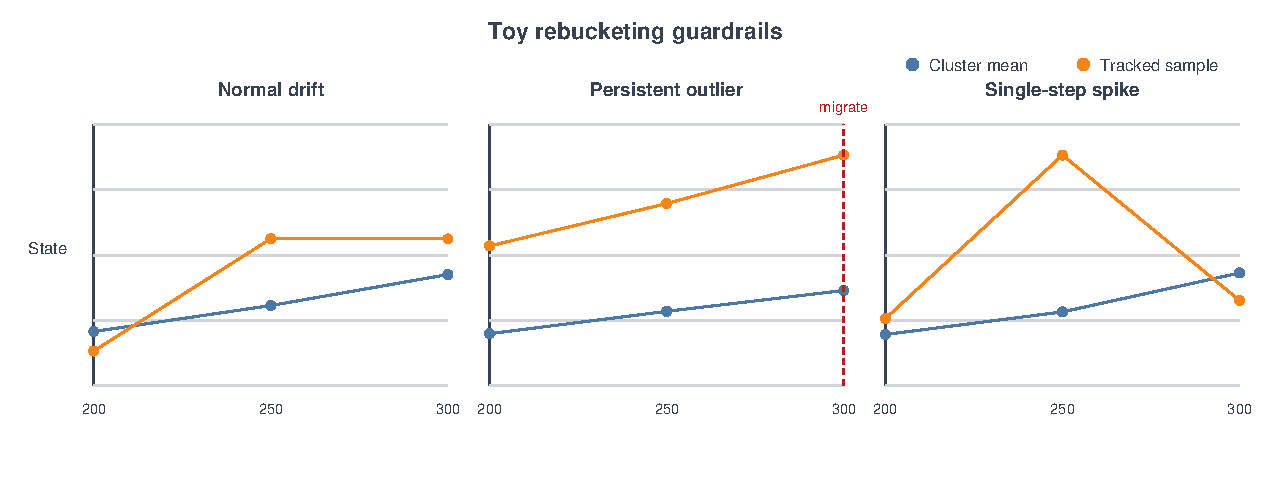
\includegraphics[width=0.95\linewidth]{figures/fig_toy_rebucket_guardrails.pdf}

  Toy simulation verifies that only persistent outliers migrate.
\end{frame}

\begin{frame}{Limitations}
  \begin{itemize}
    \item Current comparisons are limited-run and do not include confidence intervals.
    \item Difficulty-only initialization may not match model competence.
    \item Re-bucketing changes task composition, not only difficulty.
    \item Experiment 2 under accuracy-based initialization is still pending.
  \end{itemize}
\end{frame}

\begin{frame}{Conclusion and Next Step}
  \begin{itemize}
    \item AES is a working learner-state-aware environment selector for Math+Zebra RL post-training.
    \item Best current conclusion: meaningful mechanism behavior, step-200 gains, and interpretable micro-bucket drift.
    \item Main next step: accuracy-based initialization plus multi-seed evaluation.
  \end{itemize}
\end{frame}

\end{document}
